\chapter{Asynchronous Byzantine Fault Tolerant: HoneyBadgerBFT}
\label{ch:hbbft}
In this chapter, we describe an Asynchronous Byzantine Fault Tolerant Consensus Protocol, i.e., The HoneyBadger of BFT Protocols (HoneyBadgerBFT) \cite{miller2016honey}. HoneyBadgerBFT is a practical asynchronous BFT protocol which can be used as a blockchain agreement protocol for both permissioned/ private and permissionless/ open blockchain to reach consensus on order of transactions in ledger.



We are defining the protocol in a modular style. Let's learn about each module, and at the end of this chapter, we will see how the following modules combine and form HoneyBadgerBFT protocol.
\section{RB: Reliable Broadcast}
\begin{figure}[!h]
    \centering
    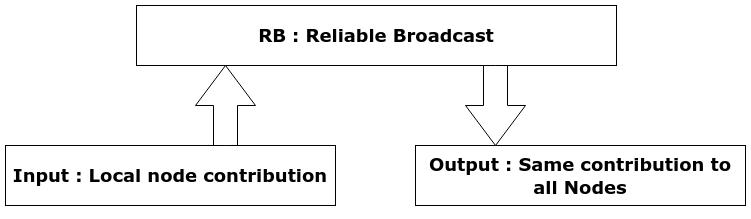
\includegraphics[scale=0.5]{images/RB.png}
    \caption{Reliable Broadcast\cite{POANetwork}}
    \label{fig:rb}
\end{figure}
The purpose of Reliable Broadcast\cite{POANetwork} \cite{bracha1987asynchronous} \cite{cachin2005asynchronous} is to broadcast its \textit{contribution} to the network even if some nodes act maliciously. To make the process of broadcasting efficient, RB uses the following process to split and encode.
\subsection{Erasure Code}
Erasure code\cite{Erasure_code} is a forward error correction code, which transforms input message into a larger message such that the original can be reconstructed from a subset of the larger message.\\
In simple words, an input message transformed and split-ed into parts (let's say 10 parts), and the original message can be recovered with only the subset of the split parts of the message(let's say 6 parts).
\subsection{Merkle Tree}
Merkle tree\cite{Merkle_tree}\cite{merkle1980protocols} is a tree build over the nodes of data. It allows secure and efficient verification of data.
\\\\
Now, When RB instance gets input, it divides the input into parts, equal to the total number of nodes in the network using \textit{erasure} coding. Then these shares are sent to their corresponding nodes. After a certain number of message exchanges between nodes, All honest nodes will eventually get enough parts to reconstruct the original message even if some nodes act maliciously. \textit{Merkle} tree is used as a small-sized proof to verify that the message received (i.e. part of \textit{erasure} code) by the node, belongs to the same tree (means belongs to the same \textit{contribution} that is being broadcasted). As these proof are very small in size, low bandwidth is required and to verify that the same message is broadcasted to all nodes.
% Merkle tree is used as a tool to verify the message content between nodes. Using Merkle tree proof, which has very small size, is used as evidence that all parts of the erasure code belong to the same message. A node can easily exchange these proofs to verify that the same message is broadcasted to all RB instances.
For more details read chapter \ref{ch:impl}

\section{BA: Binary Agreement}

\begin{figure}[!h]
    \centering
    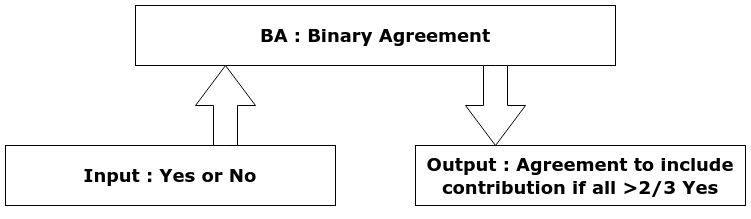
\includegraphics[scale=0.5]{images/BA.png}
    \caption{Binary Agreement\cite{POANetwork}}
    \label{fig:ba}
\end{figure}
Binary Agreement\cite{10.1145/2611462.2611468}\cite{POANetwork} is the core of the agreement process of HoneyBadgerBFT. This algorithm decides whether a contribution in subset is to be included in final output or not.
The output and input of this algorithm is a binary value (1 or 0).

This agreement process may require multiple rounds to conclude. This algorithm accounts for multiple factor that can change the outcome like getting different votes from different nodes.

\textit{BA} produces an output once at least two-third nodes agree on the same value either 1 or 0 i.e. to include the contribution or not.
For more details read chapter \ref{ch:impl}

\section{Subset}
\begin{figure}[!h]
    \centering
    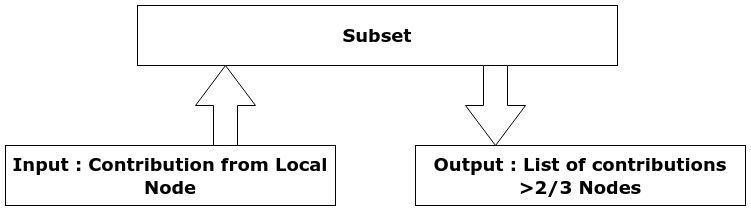
\includegraphics[scale=0.5]{images/Subset.png}
    \caption{Subset\cite{POANetwork}}
    \label{fig:subset}
\end{figure}
\textit{Subset}\cite{ben1994asynchronous}\cite{POANetwork} is the main functional unit of HoneyBadgerBFT consensus protocol. Each \textit{Subset} gets input from its \textit{HB} instance and returns the subset of inputs on which all honest \textit{Subsets} agree.
It receives the input i.e. \textit{contribution} from \textit{HB}. \textit{Subset} uses \textit{RB} instances to broadcast its \textit{contribution} to all nodes as well as receive other nodes' \textit{contributions}.


\textit{Subset} creates \textit{RB} instances for each node in the network. Each \textit{Subset}  provides input to only one \textit{RB} instance (Node 1's subset will provide input to RB instance 1, Node 2's subset to RB instance 2 and so on) and wait for \textit{RB} instances to finish
To confirm if the all \textit{RB} instances have finished and to decide whether to include the output in the final list, \textit{Subset} uses \textit{BA} instances. It instantiates the Binary Agreement algorithm for each node similar to \textit{RB} instances.  It provides input to \textit{BA} instance `1' or `0' based on whether the corresponding instance of \textit{RB} has finished or not.


Upon completion of all \textit{BA} instances, the \textit{Subset} algorithm makes a list of all contributions. It includes the contribution from \textit{RB} instance only if its corresponding \textit{BA} instance output is 1.
Then \textit{Subset} sends the list of \textit{contributions} agreed-upon back to \textit{HB}.
List of contributions contains at least $N-f$ contribution, where $f$ : Number of faulty and nodes $N$ : total number of nodes.
For more details read chapter \ref{ch:impl}

\section{HB:  HoneyBadger}
\label{sec:HB_1}
\begin{figure}[!h]
    \centering
    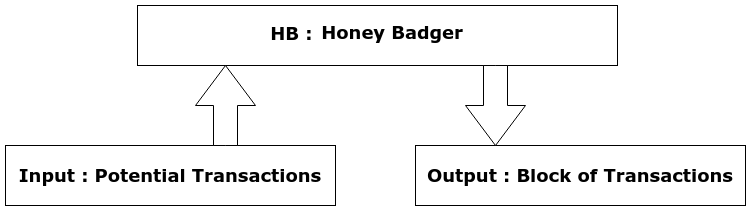
\includegraphics[scale=0.7]{images/QHB.png}
    \caption{Honey Badger\cite{POANetwork}}
    \label{fig:qhb}
\end{figure}
HoneyBadger\cite{POANetwork} is the top-level algorithm, and it takes transaction as input and after consensus return batch of transactions as output. Each node in the network runs only a single instance of HB, and all other modules such as \textit{subset}, \textit{BA}, and \textit{RB} are contained and run within that instance of HB.

Within each node, HB maintains a buffer of pending transactions it received. These transactions are sent by the client for ordering to the orderer node.
These transactions can be of any type.
HB  randomly selects transactions from the top of the buffer; these randomly selected transactions are called \textit{contribution}; the size of the contribution is selected to make message transfer efficient. Let block size B and the total number of nodes be N, and then the contribution size will be B/N. Random selection ensures the chances of the duplicate transactions are low.

HB makes progress in epochs, It provides one contribution as input per epoch to \textit{Subset} instance for that epoch. After providing input \textit{HB} wait for the output from \textit{Subset}.

The output received is a list of contributions provided and agreed upon by all \textit{Subset} instances in the network. To prepare a block, HB removes the duplicate transactions from the list and sort them. It also removes transactions the overlapping transactions from the buffer that are present in the block.

The finalized block is then the output for this epoch, and the process begins all over again.
For more details read chapter \ref{ch:impl}

\section{The Honey Badger Transaction Flow}
\begin{figure}[!h]
    \centering
    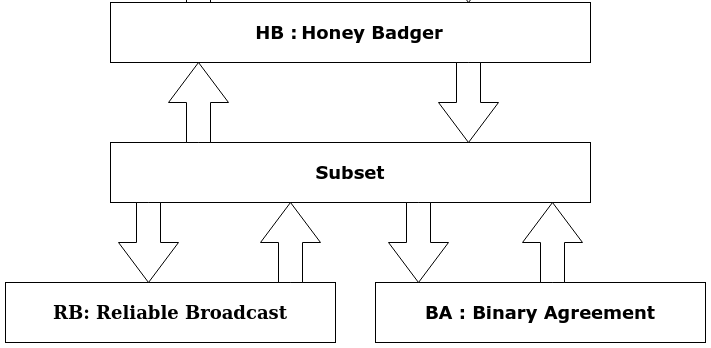
\includegraphics[scale=0.7]{images/overall.png}
    \caption{Overall HoneyBadger Protocol\cite{POANetwork}}
    \label{fig:overall}
\end{figure}

Now let's look at the overview of the whole protocol by looking at the transaction flow in HoneyBadgerBFT.


When a client sends a \textit{transaction} to HoneyBadgerBFT instance, it is added to the queue of the pending transactions. After some time, \textit{HB} selects random transactions for the current epoch; the \textit{transaction} gets picked up and included in the \textit{contribution}. The \textit{contribution} is then submitted to the \textit{Subset} instances, Which passes this \textit{contribution} to \textit{RB} to broadcast it to all the nodes in the network. After the completion of \textit{RB} instance for this contribution. \textit{Subset} provides `$1$' as input to \textit{BA} instance, and if \textit{BA} for this contribution completes with `$1$' as output. Then this \textit{contribution} is included in the list of selected \textit{contributions} for this epoch. And when \textit{HB} gets output from \textit{Subset}, it converts the output to block, and the \textit{transaction} gets committed. 